Este estudo propõe a identificação de árvores de embaúba, por meio de imagens, utilizando uma Convolutional Neural Networtk (CNN) para diferenciá-las de outras espécies arbóreas. A abordagem automatizada reduz a dependência de métodos manuais, dispendiosos e demorados, comumente empregados em inventários florestais. As Redes Neurais Artificiais (RNAs) são sistemas inspirados no cérebro humano, desenvolvidos para criar máquinas capazes de aprender e realizar tarefas complexas. Pioneiros como \cite{mcculloch1943logical} criaram o primeiro modelo de neurônio artificial, conhecido como Logical Threshold Unit (LTU), que executava funções lógicas simples, estabelecendo as bases para o desenvolvimento das RNAs. Essas redes simulam a capacidade de aprendizado do cérebro humano, dividindo-se em dois aspectos principais: a arquitetura, que define como as unidades de processamento estão conectadas, e o aprendizado, que ajusta os pesos das redes conforme novas informações são processadas.

Com o crescimento no volume de dados disponíveis e o avanço dos processadores, as RNAs evoluíram para redes profundas (Deep Networks - DN), que têm superado outros algoritmos de aprendizado de máquina em tarefas como reconhecimento de imagens, voz e linguagem natural. Dentre essas redes, as Redes Neurais Convolucionais (Convolutional Neural Networks - CNN) destacam-se pelo desempenho notável em reconhecimento de imagens, sendo inspiradas no processamento visual do cérebro para extrair padrões cada vez mais complexos. 

\subsection*{AMBIENTE DE TREINAMENTO}
Foi utilizado um hardware composto por um processador Intel(R) Core(TM) i7-9700K CPU 3.60GHz, 16 GB de memória RAM DDR4 e uma placa de vídeo NVIDIA GeForce GTX 960 com 4GB de memória DDR5. Essa configuração garantiu o treinamento dos modelos em tempo hábil, permitindo o ajuste das variáveis de entrada para o aperfeiçoamento do modelo.
Para a implementação do algoritmo de identificação de espécies arbóreas, foi construído um dataset contendo:
\begin{itemize}
    \item 90 imagens da classe embaúba(Cecropia spp.), coletadas em trabalho de campo pelos autores;
    \item 310 imagens de outras espécies arbóreas, obtidas de banco de imagens públicas, que serviram como classe de controle.
\end{itemize}

\subsection*{IMPLEMENTAÇÃO DO ALGORITMO TENSORFLOW}

Visando classificar automaticamente essas categorias, adotou-se uma CNN com arquitetura personalizada, composta por:

\begin{itemize}

    \item Três camadas convolucionais, com 32, 64 e 64 filtros (kernels 3x3), respectivamente;
    \item Camadas de MaxPooling (2x2) para redução dimensional;
    \item Funções de ativação ReLU (para não-linearidade) e Softmax (para classificação).
   
\end{itemize}

A - Camada de Entrada: Representada por um tensor bidimensional com dimensões 918x918 pixels de altura e largura.
B - 1ª Camada convolucional onde foram aplicados 32 filtros com kernel 3x3 a fim de extrair padrões visuais locais como bordas e texturas simples, resultando em um novo tensor, de mesmas dimensões, com 32 canais de ativação.


\begin{figure}[!h]
    \centering
    \caption{Evolução da acurácia ao longo dos treinamentos}
    \label{Gráfico 3}
    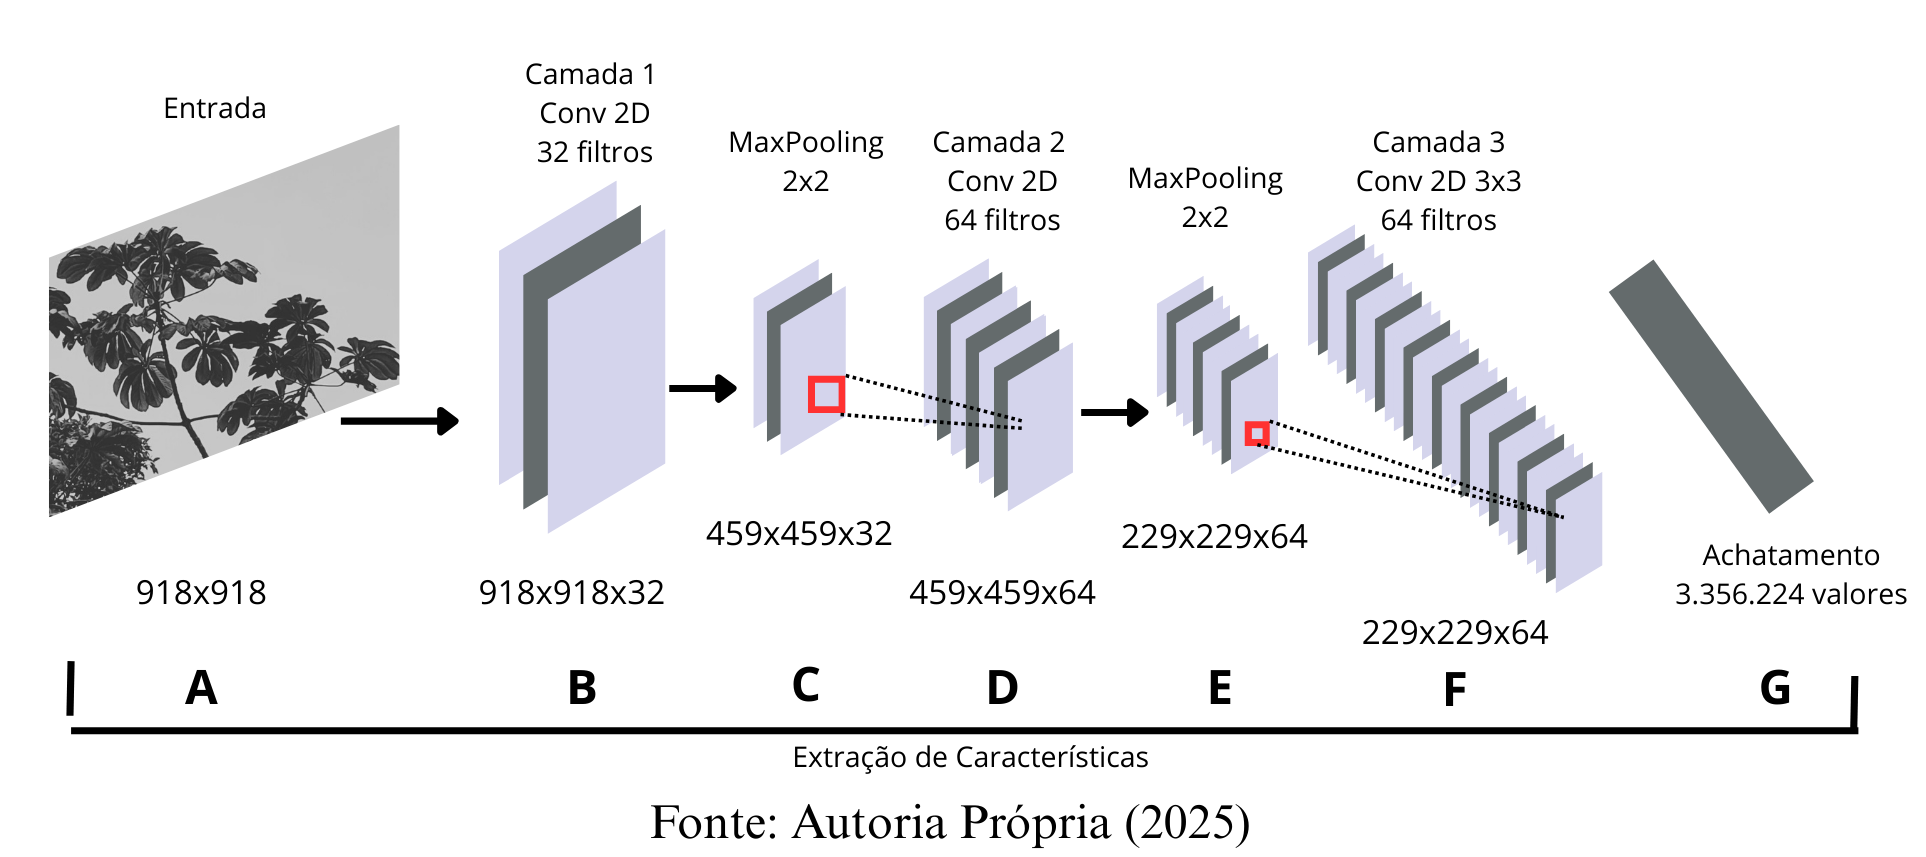
\includegraphics[width=0.9\linewidth]{Illustrations/tensorflow1.png}
\end{figure}

C - 1ª Camada MaxPooling em que aplicou-se pooling  com janelas 2x2, reduzindo a altura e largura pela metade. A redução das dimensões também auxilia a redução da complexidade computacional. O resultado é um tensor de 459x459 pixels e 32 canais de ativação.

D - 2ª Camada Convolucional. Nesta etapa aplicou-se 64 filtros 3x3, para detectar padrões mais complexos formados a partir das ativações da camada anterior.

E - 2ª Camada MaxPooling. Novamente reduziu-se as dimensões para reduzir a complexidade computacional.

F - 3ª Camada Convolucional, em que foram aplicados 64 filtros 3x3 para obter características ainda mais abstratas e específicas da imagem.
G - Camada Flatten(Achatamento). Converteu-se o tensor tridimensional em um vetor unidimensional totalizando 3.356.224 elementos.

H - Camada Densa com ReLU. Nesta camada totalmente conectada, recebeu o vetor e aplicou-se a função de ativação ReLU, que adiciona não-linearidade, que permite o aprendizado de combinações complexas de características.

\begin{figure}[!h]
    \centering
    \caption{Evolução da acurácia ao longo dos treinamentos}
    \label{Gráfico 3}
    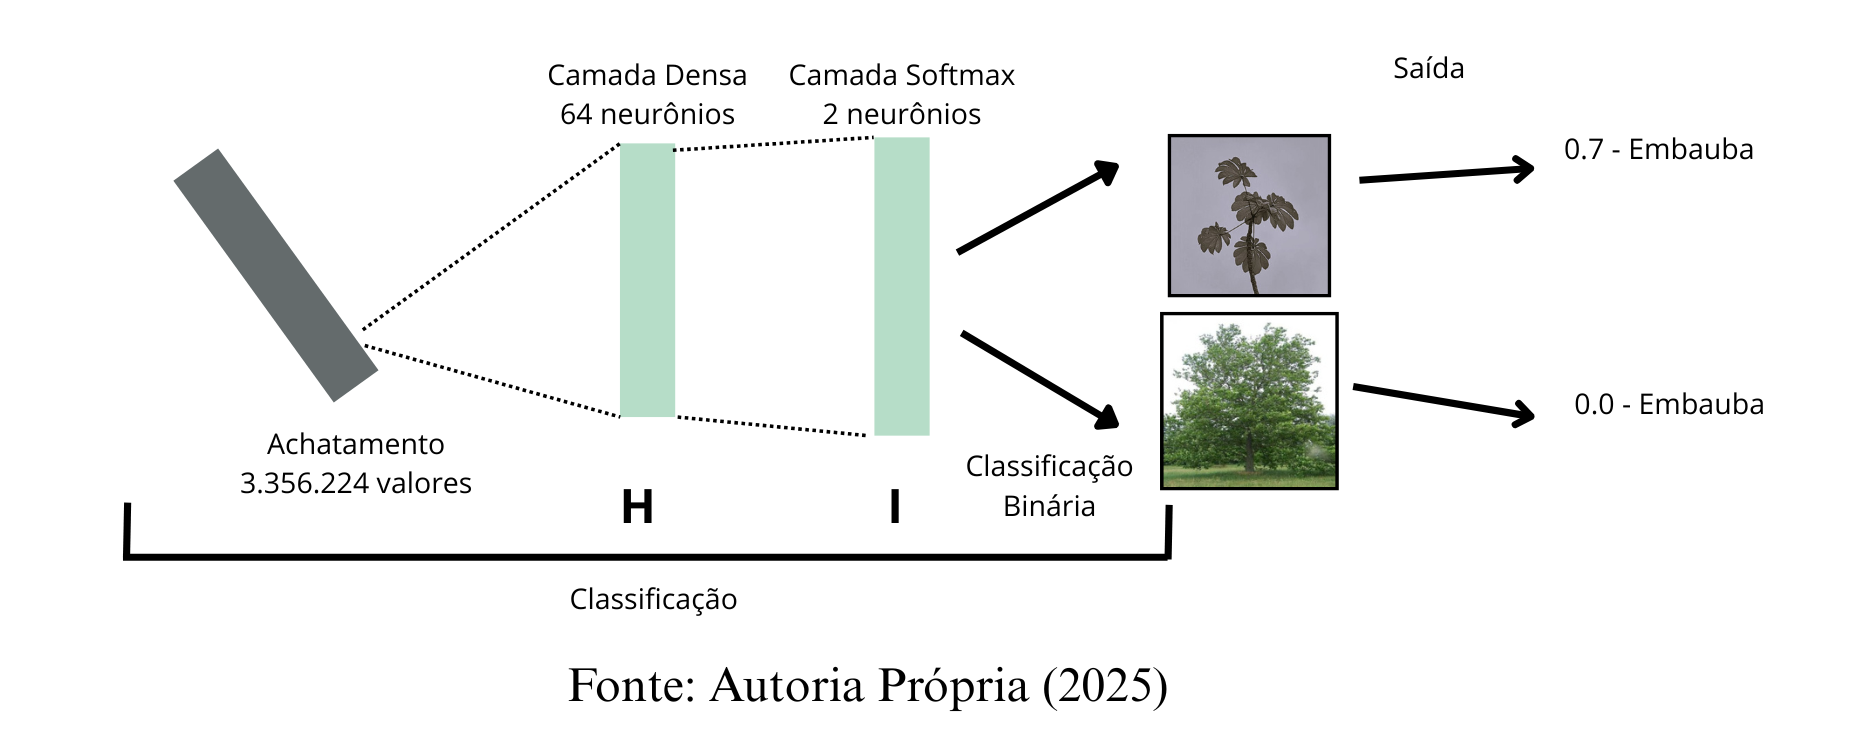
\includegraphics[width=0.9\linewidth]{Illustrations/tensorflow2.png}
\end{figure}

I - Camada de Saída com \textit{SoftMax}. Nesta camada final, classifica-se a imagem em uma das categorias possíveis, convertendo valores em probabilidades, indicando a classe mais provável.

A escolha por uma CNN customizada - em vez de modelos pré-treinados como VGG ou ResNet - justifica-se pelo tamanho reduzido do dataset de 400 imagens, evitando assim o \textit{overfitting} (sobreajuste do modelo de dados de treinamento). O treinamento foi realizado do zero (\textit{from scratch}), sem transferência de aprendizado, para garantir a adaptação do modelo às características específicas das imagens coletadas. 
A fim de verificar como o modelo generaliza para dados novos, ou seja, como ele se comporta com dados que não foram usados durante o treinamento, utilizou-se a validação cruzada(\textit{K-Fold Cross Validation}). Neste método, os dados são divididos em K partes iguais, posteriormente ele é treinado K vezes, e a cada iteração é utilizado uma dessas partes como conjuntos de teste até completar todos. A métrica de desempenho é calculada 4 para cada uma das K execuções e ao final é feita a média desse valores.

O procedimento de avaliação do modelo envolve validação cruzada com 10 folds, visando garantir a robustez e a capacidade de generalização do modelo. O dataset é dividido em 10 partes, e o modelo é treinado e validado 10 vezes, utilizando, a cada rodada, uma parte distinta para validação enquanto as outras nove são usadas para treinamento.
O modelo é compilado com o otimizador Adam e treinado utilizando a função de perda \textit{Sparse Categorical Crossentropy}, apropriada para tarefas de classificação multiclasses com rótulos inteiros. A entropia cruzada calcula o erro comparando as probabilidades atribuídas pelo modelo a cada classe (saída) com as probabilidades reais (valores desejados), normalmente representadas por "1" para a classe correta e "0" para as demais. O objetivo é minimizar essa perda para que o modelo faça previsões mais precisas.

Com intuito de garantir que a rede neural seja confiável, seu aprendizado deve ser refinado gradualmente. Para tanto, o conjunto de dados é treinado várias vezes, denominando-se épocas, ou epoch em inglês. Durante o treinamento, são realizadas 100 épocas para assegurar que o modelo tenha tempo suficiente para aprender as características dos dados, com batch size definido como 32. A métrica de desempenho adotada é a acurácia, que mede a proporção de previsões corretas do modelo. Os valores de acurácia para cada fold são coletados, e a acurácia média é calculada para avaliar o desempenho geral do modelo.

\subsection*{IMPLEMENTAÇÃO DE APLICAÇÃO MOBILE PARA VISUALIZAÇÃO DE RELATÓRIOS}

Para o desenvolvimento de um sistema de visualização de relatórios de identificação de árvores em ambiente mobile, a aplicação será construída em React Native, proporcionando uma interface intuitiva e responsiva dada sua eficiência e versatilidade para criação de aplicações destinadas a múltiplas plataformas\cite{(ALMEIDA, 2024)}. Esta interface permitirá que os usuários naveguem pelos relatórios dentro da tela de análises (b). No relatório (d), são apresentados informações relacionadas à Embaúba e seus pontos cartesianos na imagem analisada. Além disso, será implementada uma função de atualização em tempo real, garantindo que as informações mais recentes processadas pela Interface de Programação de Aplicações (\textit{Application Programming Interface} - API) sejam refletidas nos relatórios. 

\begin{figure}[!h]
    \centering
    \caption{Evolução da acurácia ao longo dos treinamentos}
    \label{Gráfico 3}
    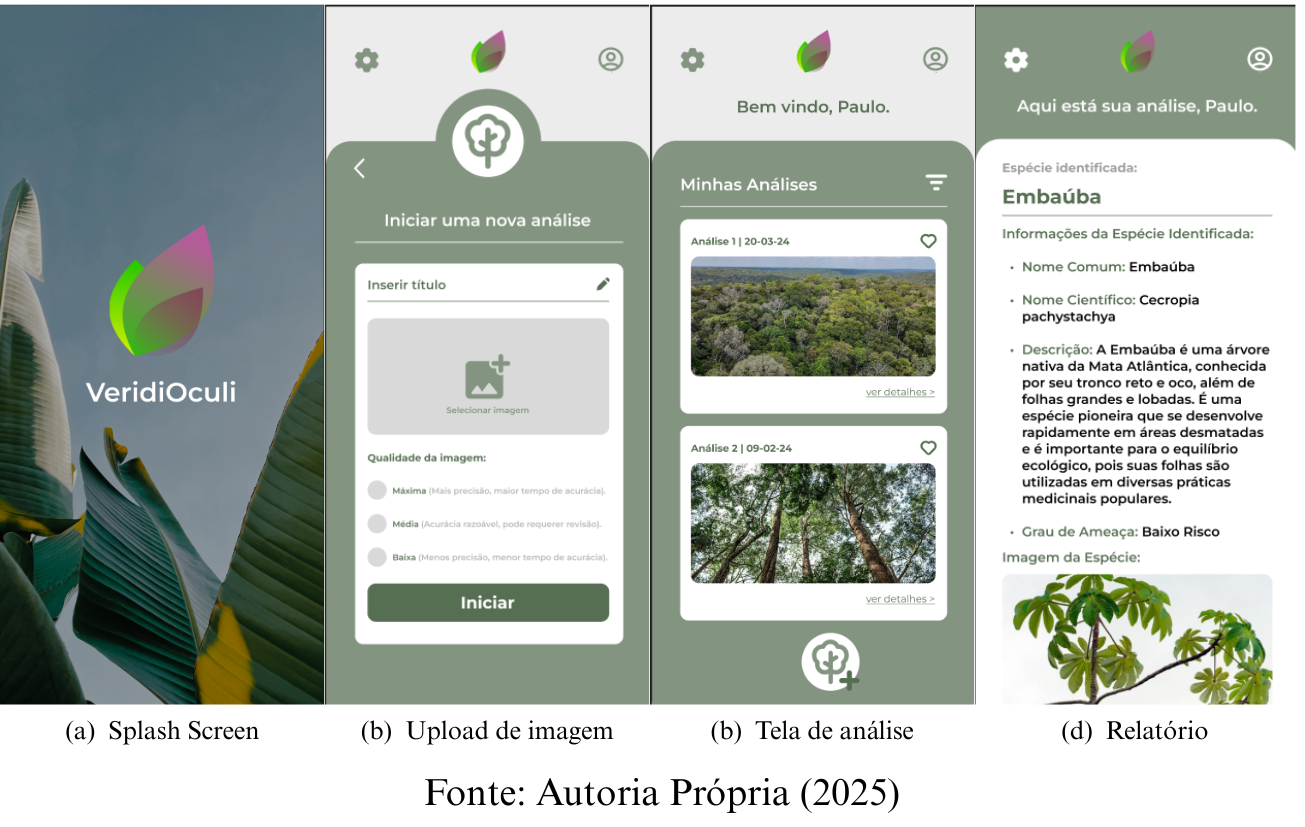
\includegraphics[width=0.8\linewidth]{Illustrations/aplicacaomobile.png}
  
\end{figure}

A API será desenvolvida em \textit{Flask} e hospedada em um ambiente de nuvem da Amazon Web Services (AWS), com dados armazenados em um \textit{bucket S3} . Esse setup em nuvem garantirá escalabilidade e alta disponibilidade, além de segurança no controle de acesso às informações. A API acessará e retornará os dados de inventário florestal conforme solicitado pela aplicação, após realizar testes de conectividade e otimizações de desempenho para melhor integração entre API e aplicação. Para validar a funcionalidade da inteligência artificial generativa utilizada na identificação das espécies arbóreas, serão realizados testes de precisão e eficiência, utilizando conjuntos de dados de teste e métodos de \textit{benchmarking}. A IA será avaliada quanto à sua capacidade de identificar corretamente espécies nativas e invasoras. Por fim, testes de integração garantirão que os relatórios gerados pela IA estejam formatados adequadamente para visualização no sistema mobile, assegurando a consistência e confiabilidade dos dados apresentados aos usuários.